\documentclass{article}
\usepackage[a4paper, hmargin={2.8cm, 2.8cm}, vmargin={2.5cm, 2.5cm}]{geometry}
%%%%%%%%%%%%%%%%%%%%%%%%%%%%%%%%%%%%%%%%%%%%%%%%%%%%%%%%%%%%%%%%%%%%%%%%%%%%%%%%

%%%%%%%%%%%%%%%%%%%%%%%%%%%%%%%%%%%%%%%%%%%%%%%%%%%%%%%%%%%%%%%%%%%%%%%%%%%%%%%%
\usepackage[utf8]{inputenc}
\usepackage[T1]{fontenc}
%%%%%%%%%%%%%%%%%%%%%%%%%%%%%%%%%%%%%%%%%%%%%%%%%%%%%%%%%%%%%%%%%%%%%%%%%%%%%%%%


%%%%%%%%%%%%%%%%%%%%%%%%%%%%%%%%%%%%%%%%%%%%%%%%%%%%%%%%%%%%%%%%%%%%%%%%%%%%%%%%
\usepackage{mathtools}
\usepackage{amsthm}
\usepackage{amssymb}
\usepackage{csvsimple}
\usepackage{subcaption}
\usepackage{url}
%%%%%%%%%%%%%%%%%%%%%%%%%%%%%%%%%%%%%%%%%%%%%%%%%%%%%%%%%%%%%%%%%%%%%%%%%%%%%%%%


%%%%%%%%%%%%%%%%%%%%%%%%%%%%%%%%%%%%%%%%%%%%%%%%%%%%%%%%%%%%%%%%%%%%%%%%%%%%%%%%
\usepackage{fancyhdr}
\usepackage{graphicx}
\usepackage{parskip}
\usepackage{listings}
\usepackage{enumitem}
\usepackage{titlesec}
\usepackage[lastpage,user]{zref}
\usepackage{caption}
\usepackage{scrextend}
\usepackage[outputdir=./.latex-out]{minted} % TODO slet hvis du ikke bruger minted
\usepackage{listings}
\usepackage{blindtext}
\pagestyle{fancy}
\lhead{\LaTeX webinar} % TODO indsæt venstre sidehoved
\rhead{Study Now} % TODO indsæt højre sidehoved
\cfoot{\thepage\ of \zpageref{LastPage}}
\setlist{nolistsep}

\newcommand{\tex}[1] {
  \mintinline{latex}{#1}
}

\title{
  \vspace{13em}
  \large{Study Now} \\
  \Large{\LaTeX webinar} \\
}

\author{
  Benjamin Rotendahl --- Benjamin@Rotendahl.dk
}

\date{
  \vspace{22em}
  \today
}

\begin{document}
\maketitle		% Forside
\thispagestyle{empty}
\newpage

\thispagestyle{empty}
\tableofcontents
\newpage % TODO indsæt indholdsfortegnelse eller slet for at fjerne

\setcounter{page}{1}

\section{Introduction}
 Dette dokument fungerer som et \emph{cheatsheet}. Det gennemgår de forskellige
 former for opsætning og funktioner i \LaTeX. Når du selv sidder og skriver, kan
 du enten bruge den færdige PDF som opslagsværk, eller kigge på kildekoden.
 Husk, at du selv kan udvide dokumentet med yderligere sektioner, hvis du finder
 nogle seje funktioner i din videre færd med \LaTeX{}.

 \subsection{\LaTeX baggrund}
   Før vi går i gang med syntaksen osv., gennemgår vi, hvordan \LaTeX{} fungerer og
   laver kildekode om til en PDF.
   \LaTeX{} er et skriftsstyringssprog, som bruges til at skrive dokumenter med. Det er
   særligt godt til at skrive dokumenter med matematik, kode og andre
   videnskablige figurer. \LaTeX er en udvidelse af TeX, som blev udgivet af Donald
   Knuth i 1989. For installationsguide se sektion~\ref{hejsa}

 \subsection{Fra kildekode til PDF}\label{hejsa}
   \LaTeX er ikke et skriveprogam, men et sprog samt compiler\footnote{
     Det, man kalder en \emph{oversætter} på dansk}. Den tager kildekoden, som
   er skrevet i en \emph{editor}, og laver det om til en PDF. En editor til
   lokalt brug kan f.eks. være \emph{Visual studio code}\cite{vscode}. Det er
   en editor, som kan bruges til at skrive alle slags sprog. Man installerer
   ekstra pakker, som udvider dens funktionalitet, f.eks. har den både pakker
   til at hjælpe med python-kode, javascript og \LaTeX{}\cite{latexPackage}.

   Efter koden er skrevet, skal den gives videre til en \emph{compiler}, som
   tager kildekoden og laver det om til en PDF. Det er compileren, som
   inkluderer filer, figuerer osv. Er der en fejl i kildekoden, gør compileren
   sit bedste for at fastslå, hvad fejlen er, og hvordan den kan fixes. Der findes
   forskellige versioner af LaTeX compileren, som prinært varierer i, hvilke
   ekstra pakker og værktøjer de inkulderer.
   ``The latex project TeX''\cite{texLive} har links til distrubtioner for de
   de forskellige styresystemer. Med en compiler og editor installeret er man
   klar til at bygge sit første latex dokument, , processen kan ses i
   figuer~\ref{fig:compile}.

   \subsubsection{Overleaf}
     Sektion~\ref{sec:local} forklarer, hvordan du opsætter dit eget miljø lokalt.
     Der findes tjenester som Overleaf\footnote{\url{overleaf.com}}, der fungerer
     på samme måde som google docs. Man arbejder i en webrowser, hvor de giver en et fuldt opsat
     miljø. Man slipper altså for at installere noget lokalt og har nemmere ved
     at dele sit arbejde med eventuelle gruppemedlemmer. Ulempen er, at man ikke
     har samme konfigurationsmuligheder som lokalt, og det kræver internetadgang
     at tilgå.
     \begin{figure}[h]
       \centering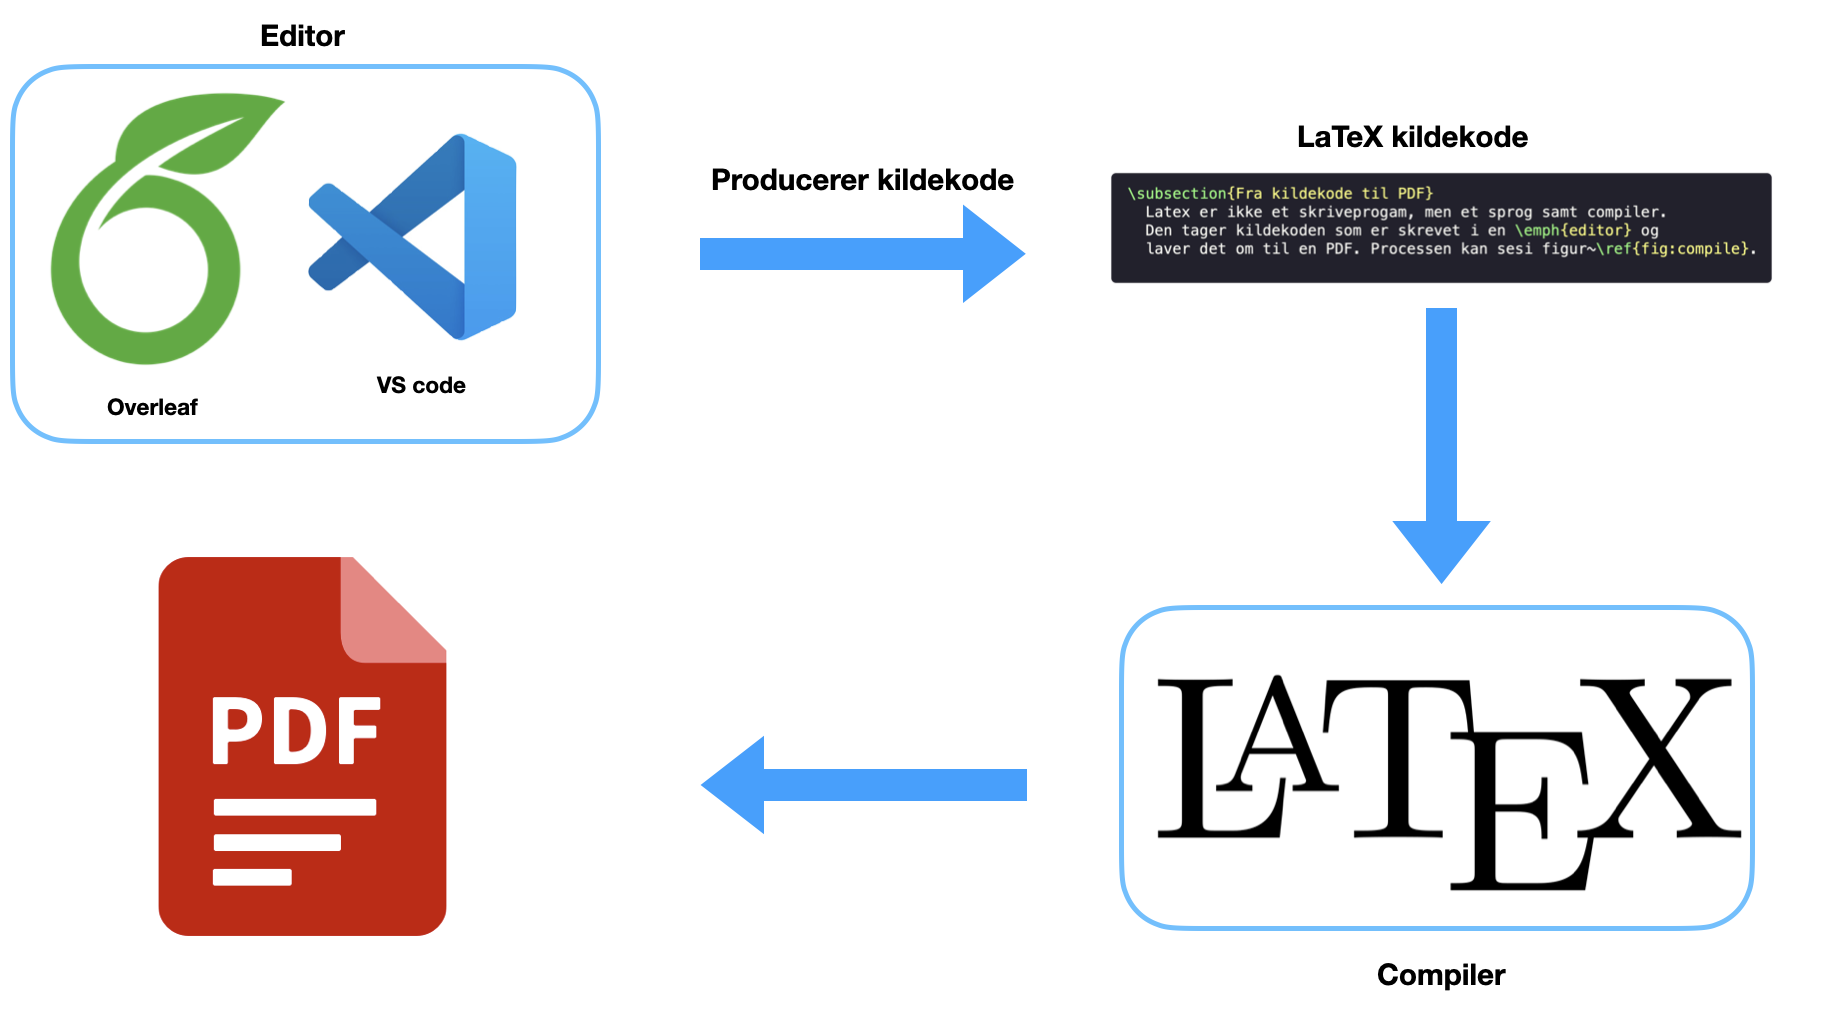
\includegraphics[width=0.9\textwidth]{assets/compile.png}
       \caption{Hvordan man kommer fra kildekode til pdf}\label{fig:compile}
     \end{figure}


   \subsubsection{Kommando syntax}
     En kommando består af en ``backslash'' efterfulgt af et kommandonavn.
     Tager kommandoen parametre, skal de skrives i krølleparanteser
     efter. F.eks. kan vi skrive \LaTeX{} ved at skrive \tex{\LaTeX}. Der findes
     genveje til de mest gængse kommandoer.
     \begin{description}
       \item[Linjeskift] \LaTeX{} sørger selv for at lave linjeskift i ens tekst.
         Laver man et manuelt linjeskift, ignorer programmet det. Det er på den måde, at man har
         bedre mulighed for selv at formattere ens kildekode, uden det påvirker den
         endelige pdf. Ønsker man selv at bestemme et linjeskift, kan man enten indsætte to
         linjeskift i sin egen kode, skrive \tex{\linebreak} eller to backslashes.
         \tex{\\}

       \item[Tvunget mellemrum] Ligesom med linjeskift, fjerner \LaTeX{} også
         nogle mellemrum. Hvis man har man sat flere end et, bliver de slået sammen til et enkelt.
         Ønsker man et tvunget mellemrum, skriver man \tex{hej ~~~ verden}

       \item[Ny side] Ønsker man at tvinge \LaTeX til at skifte til en ny side,
         skriver man \tex{\newpage}

       \item[Anførselstagn] Ønsker man at sætte tekst i ``anførselstegn'', gøres
         det ved at skrive \tex{``anførselstegn''}

       \item[Kommentar] Ønsker man at inkuldere noget tekst i sin kildekode, men
         ikke i den færdige pdf, kan man lave en \emph{Kommentar}. Det er brugbart
         for at lave påmindelser til sig selv eller gruppemedlemmer. Sætter man
         et \(\%\) tegn, vil resten af linjen ikke blive inkluderet. For at
         skrive \(\%\), sætter man så en backslash foran \tex{\%}


       \item[Matematik] Der findes to måder at skrive matematik på, den ene er
         \emph{inline}, hvor matematikken står inde i teksten, f.eks. \(x^2 +4\),
         hvilket gøres ved at skrive \tex{\(x^2 +4\)}. Den anden er \emph{display}
         mode, hvor matematikken står udenfor teksten, det skrives sådan her:
         \tex{\[x^2 +4\]}. f.eks \[x^2 +4\]
       \item[Miljøer] Ved større kommandoer kan det blive svært at skrive det
         hele i krølleparanterser bagefter. Til sådane kommandoer kan man skrive det
         med miljønotation. Ønkser vi f.eks. at have en linje i midten, kunne
         vi skrive \tex{\centering{\\ Jeg er i midten \\}}.
         \centering{\\ Jeg er i midten \\}
         Var min tekst længere, ville det være nemmere at skrive
         \begin{minted}[tabsize=1]{latex}
					\begin{center}
						Jeg er en længere tekst, der står i miden af dokumentet
					\end{center}
				 \end{minted}
         Der findes mange miløjer til at lave alt fra lister, matricer, tabeller,
         figurer osv.

     \end{description}

     \begin{flalign}
       f(x, y)                       & = 3x^2y + 3y^2 \\
       \frac{\partial f}{\partial x} & = 6xy          \\
       \mathbf{z}                    & =
       \begin{bmatrix}
           2 & 2 & 3 \\
           3 & 4 & 5 \\
           6 & 7 & 8 \\
         \end{bmatrix}                                 \\
       \mathbf{z}                    & =
       \begin{bmatrix}
           1      & \dots  & n      \\
           \vdots & \ddots & \vdots \\
           n      & \dots  & n      \\
         \end{bmatrix}                       \\
         \left ( 1 + \frac{1}{4} \right )^2
     \end{flalign}


     \begin{description}
       \item[p1 hej] punkt 1
       \item[p2 hej] punkt 2
       \item[p3 hej] punkt 3 \begin{description}
           \item hej med jer
           \item farvel med jer
         \end{description}
     \end{description}


     \begin{table}[h]
       \centering
       \begin{tabular}{||c c | c c||}
         \hline
         søjle1 & søjle2 & søjle4 & søjle4 \\  \hline
         1      & 6      & 87837  & 787    \\
         2      & 7      & 78     & 5415   \\
         3      & 545    & 778    & 7507   \\
         4      & 545    & 18744  & 7560   \\
         5      & 88     & 788    & 6344   \\
         \hline
       \end{tabular}
       \caption{Eksempel på manuelt skrevet tabel}\label{table:data}
     \end{table}

     \newpage
     \appendix
     \bibliography{assets/references}{}
     \bibliographystyle{plain}


\end{document}
